%% ============================================================
%% Concord: Cooperative Query Optimization for LLM Agent
%%          Database Sessions
%%
%% Target venue: SIGMOD/VLDB (currently set up as acmart sigconf;
%%               swap to pvldb class when venue is finalized)
%% ============================================================

%% --- Title alternatives (uncomment to swap) --------------------
%% Concord: Cooperative Query Optimization for LLM Agent Database Sessions
%% Covenant: A Declared-Intent Protocol for Agent-Database Cooperation
%% Agora: Shared Workspaces for Cooperative LLM Agent SQL Sessions
%% Declared-Intent Cooperation: Optimizing LLM Agent Database Sessions at the Protocol Layer
%% ---------------------------------------------------------------

\documentclass[sigconf, nonacm, review]{acmart}

%% acmart options explained:
%%   sigconf  -- SIGMOD/ACM conference two-column style
%%   nonacm   -- suppress ACM rights/permissions block while drafting
%%   review   -- line numbers on (remove for submission)

\settopmatter{printacmref=false, printfolios=true}

%% --- Packages -------------------------------------------------
\usepackage{booktabs}
\usepackage{graphicx}
\usepackage{amsmath}
\usepackage{amssymb}
\usepackage{xcolor}
\usepackage{tikz}
\usetikzlibrary{arrows.meta, positioning, shapes.geometric, calc, fit, backgrounds}
\usepackage{xspace}

%% --- Numerical macros (update these as measurements land) -----
\newcommand{\TODO}[1]{\textcolor{red}{\textbf{[TODO: #1]}}}
\newcommand{\placeholder}[1]{\textcolor{orange}{\textbf{??}\xspace}}

%% Measured numbers (current IMDB M1 post-hoc)
\newcommand{\adoptionRate}{75\%\xspace}           % voluntary save rate
\newcommand{\saveCteRate}{50\%\xspace}            % of reps using SAVE_CTE
\newcommand{\mTwoDeclRate}{45\%\xspace}           % reps emitting M2 declarations
\newcommand{\mTwoPrecision}{100\%\xspace}         % declared variants actually issued
\newcommand{\imdbSpeedupPostHoc}{1.30$\times$\xspace}    % measured, 20-rep IMDB
\newcommand{\imdbReuseSpeedup}{2.1$\times$\xspace}        % reuse-only queries
\newcommand{\imdbSingleRefSpeedup}{5.7$\times$\xspace}    % single-ref CTE subset
\newcommand{\imdbMultiRefSpeedup}{1.4$\times$\xspace}     % multi-ref CTE subset
\newcommand{\taskCompletionIMDB}{20/20\xspace}    % task completion

%% Projected / unmeasured numbers (TODO: replace when measured)
\newcommand{\imdbSpeedupPreHoc}{\placeholder{}}   % TODO: measure post pre-hoc impl
\newcommand{\imdbSpeedupFull}{\placeholder{}}     % TODO: measure with M1+M2+M3
\newcommand{\ibSpeedup}{\placeholder{}}           % TODO: InsightBench headline
\newcommand{\ibQualityAgreement}{\placeholder{}}  % TODO: rubric agreement rate

%% --- Title and authors ----------------------------------------
\title{Concord: Cooperative Query Optimization for LLM Agent Database Sessions}

\author{Pratyoy}
\affiliation{%
  \institution{Institution TBD}
  \country{USA}
}
\email{email@tbd.edu}

%% --- Abstract -------------------------------------------------
\begin{abstract}
LLM agents now run extended analytical sessions against relational databases, issuing dozens of queries against a shared working set over the course of a single task. Existing cooperative database mechanisms---materialized views, recycler-style result caching, classical multi-query optimization, adaptive indexing---were designed under the assumption that reuse opportunities must be \emph{inferred} from workload history. LLM agents, however, expose structured intent directly: they can \emph{declare} which results will be reused, and which queries will follow.

This paper presents Concord, a protocol and session-level execution harness that converts declared intent into end-to-end session speedup. Concord comprises three cooperating mechanisms: a session workspace with named result handles materialized at first execution (M1), a $k$-query lookahead declaration enabling cross-query co-materialization and lookahead-aware physical property synthesis (M2), and reuse-aware physical tuning of the workspace (M3). Each mechanism is enabled by a specific declaration the agent emits; none is safely implementable from inferred intent alone. We position Concord as extending the intra-query reuse already provided by modern query engines (e.g., PostgreSQL~16's multi-reference CTE auto-materialization) to inter-query reuse across the agent's session.

We evaluate Concord on two benchmarks: 20 multi-step analytical sessions on IMDB/JOB, and \placeholder{} curated tasks from InsightBench. Across the IMDB suite, agents voluntarily adopt the workspace at \adoptionRate, Concord yields \imdbSpeedupFull end-to-end session speedup over a protocol-na\"{\i}ve baseline, and blinded rubric grading confirms equal analytical quality \ibQualityAgreement. On InsightBench, Concord yields \ibSpeedup session speedup. We release Concord as an extension-free harness over unmodified PostgreSQL~16.
\end{abstract}

\keywords{LLM agents, query optimization, materialization, multi-query optimization, cooperative databases}

\begin{document}

\maketitle

\section{Introduction}
\label{sec:intro}

LLM agents have emerged as a new class of database client. Unlike human analysts, who issue queries irregularly as analytical intuition develops, agents follow systematic task-decomposition patterns: they establish a working dataset, then issue a sequence of aggregations, filters, and breakdowns against it. Across a recent characterization of agent sessions on analytical workloads, we observe that the same plan-critical subexpressions recur at strikingly high rates within a session, and that the agent frequently telegraphs its next several queries in its chain of thought before executing them. This regularity is not incidental---it is a direct consequence of how modern LLM agents are trained and prompted to decompose analytical tasks.

This regularity is an optimization opportunity that existing cooperative database mechanisms are poorly equipped to exploit. Materialized views, result recyclers~\cite{ivanova2010recycler}, adaptive indexing~\cite{idreos2007cracking}, and classical multi-query optimization~\cite{sellis1988mqo,roy2000mqo} all share a common design assumption: that reuse opportunities must be \emph{inferred} from observed workload history, after enough statistics have accumulated to justify the materialization or rewriting decision. This assumption is fundamental---it governs what the database is allowed to do, when, and at what cost. Under it, a database is reactive by necessity: it can only discover reuse after paying for it at least once.

LLM agents invalidate this assumption. An agent operating under a cooperation protocol can \emph{declare} its intent prospectively: which results will be reused, which queries will follow, which physical access patterns will dominate. Given such declarations, a far richer space of optimizations becomes \emph{legal}---not merely heuristic. A result that the agent declares will be reused can be materialized on first execution without waiting for recurrence to prove the value. A set of queries the agent declares it will issue next can be co-optimized as a batch, their shared subexpressions materialized once, their physical properties synthesized from the union of their access patterns. None of this is safe under inferred intent; all of it is safe under declared intent.

\paragraph{Extending reuse across the session.}
Modern query engines already provide \emph{intra-query} reuse for free. PostgreSQL 16's multi-reference CTE auto-materialization, for instance, detects common subexpressions \emph{within} a single query and materializes them once. What has been missing is \emph{inter-query} reuse---sharing materialized state across the sequence of queries that constitutes an agent's session. Concord provides exactly this extension: a session-scoped workspace, addressable by declared names, whose contents persist across the agent's query sequence and are optimized using the agent's declared reuse and lookahead intent.

\paragraph{Three cooperating mechanisms.}
Concord consists of three mechanisms, each enabled by a specific declaration:

\begin{itemize}
\item \textbf{M1: Declared materialization.} The agent emits \texttt{-- WILL\_SAVE} before a query whose result will be reused, or \texttt{-- WILL\_SAVE\_CTE} to mark a named CTE body within a larger query as the reusable fragment. The session harness materializes the declared result on first execution via \texttt{CREATE TEMP TABLE AS}, eliminating the double-execution cost of a post-hoc save.

\item \textbf{M2: Lookahead-informed multi-query optimization.} The agent emits \texttt{-- LOOKAHEAD} declaring its next $k$ queries. The harness identifies common subexpressions across the declared window, co-materializes them once with physical properties (sort order, partial aggregates, covering columns) synthesized from the union of declared access patterns, and rewrites the declared queries to exploit the shared result.

\item \textbf{M3: Reuse-aware physical tuning.} The harness adapts session-level GUCs (e.g., \texttt{work\_mem}, parallelism) to the declared workspace's characteristics, and chooses clustering and partial-aggregate options from the declared access pattern.
\end{itemize}

Concord is implemented as a session harness over \emph{unmodified} PostgreSQL 16: no extensions, no planner patches. The declared-intent protocol is delivered through SQL comments and a small PL/pgSQL workspace catalog. This deliberately minimal integration surface is itself a design claim: if the protocol requires deep database modifications, its deployability story is weak.

\paragraph{Contributions.}
We make four contributions:

\begin{itemize}
\item A declared-intent protocol for cooperative agent-database optimization, with explicit legality conditions stating what each declaration entitles the database to do that it could not safely do otherwise (Section~\ref{sec:protocol}).

\item An empirical characterization of agent adoption and predictability on IMDB/JOB: \adoptionRate voluntary save rate across 20 multi-step analytical sessions with no explicit reward for saving, \mTwoPrecision M2 declaration precision, and a detailed picture of \emph{when} agents declare intent faithfully versus \emph{when} they iterate on the base definition in ways that defeat reuse (Section~\ref{sec:motivation}, \ref{sec:eval}).

\item A cost-model result establishing that lookahead-informed shared materialization is never worse than ad-hoc per-query optimization under stated assumptions on declaration fidelity (Section~\ref{sec:protocol}).

\item An end-to-end evaluation showing Concord yields \imdbSpeedupFull session speedup on IMDB/JOB and \ibSpeedup on InsightBench at equal analytical quality, with the speedup net of PostgreSQL 16's existing intra-query CTE materialization (Section~\ref{sec:eval}).
\end{itemize}

\paragraph{Paper organization.}
Section~\ref{sec:related} situates Concord against four prior cooperative-database traditions. Section~\ref{sec:motivation} presents the workload characterization that motivates the protocol, including a negative result on cardinality-feedback optimization for agent workloads that clarifies why the opportunity lies at the session level rather than at the single-query level. Section~\ref{sec:protocol} formalizes the protocol, the three mechanisms, and the cost model. Section~\ref{sec:impl} describes the implementation over PostgreSQL 16. Section~\ref{sec:eval} reports the empirical evaluation. Section~\ref{sec:discussion} discusses failure modes and generalization; Section~\ref{sec:conclusion} concludes.

\section{Related Work}
\label{sec:related}

Concord draws on four lines of prior work: materialized views and result caching, classical multi-query optimization, adaptive physical tuning, and recent LLM-for-database systems. We discuss each in turn, emphasizing the design assumption each makes about how reuse opportunities are discovered.

\subsection{Materialized Views and Result Caching}

Materialized views~\cite{halevy2001mv, goldstein2001mv} and result recyclers~\cite{ivanova2010recycler,nagel2013recycling} maintain precomputed results that later queries can be rewritten against. The core technical challenges have been view-matching---determining whether a stored result can answer a query~\cite{goldstein2001mv}---and maintenance under updates~\cite{gupta1995mvmaint}. MonetDB's recycler~\cite{ivanova2010recycler} and related systems~\cite{phan2008predictableperf} demonstrate that operator-level intermediate caching can yield substantial speedups on workloads with repeated subexpressions.

These systems are designed for workloads in which reuse opportunities must be discovered from observed history. Their decisions are reactive: a result is recycled when its reuse likelihood, estimated from workload statistics, justifies the storage and maintenance cost. Concord inverts this: the agent \emph{declares} which result will be reused, so the materialization decision is made at first execution, without requiring statistical evidence of recurrence. This is not a claim that declared intent is universally better---it is a claim that when the client can be trusted to declare faithfully, a richer optimization space becomes legal. Section~\ref{sec:protocol} makes the legality argument precise.

\subsection{Classical Multi-Query Optimization}

Multi-query optimization (MQO)~\cite{sellis1988mqo,roy2000mqo,dalvi2001pipelined} identifies common subexpressions across a known batch of queries and generates a shared plan that evaluates them together. MQO has been studied both as a static batch problem~\cite{roy2000mqo} and in pipelined~\cite{dalvi2001pipelined} and online~\cite{silva2012onlinemqo} settings. Recent work~\cite{mqo2020revisit} has revisited MQO in the context of modern analytical workloads.

MQO classically assumes a \emph{static} batch of queries known in advance. Concord's M2 mechanism is closer in spirit to pipelined and online MQO: the agent declares a $k$-query lookahead window ahead of execution, and the harness co-optimizes within that window. What distinguishes Concord is not the shared-plan construction itself, which builds on established MQO techniques, but the signal used to identify the batch: an explicit lookahead declaration from the agent, rather than a scheduler buffering concurrent queries. This signal carries additional structure---the agent's declared \emph{diff clauses} between lookahead queries identify exactly which predicates and group-bys vary---that a scheduler observing only the query text cannot recover without further analysis.

\subsection{Adaptive Physical Tuning}

Database cracking~\cite{idreos2007cracking} and its descendants~\cite{idreos2011crackingupdates,petraki2015holistic} adapt physical structure (sort orders, indexes) from query predicates observed at runtime. Soft indexes~\cite{graefe2010softindex} and adaptive merging~\cite{graefe2010adaptivemerge} generalize the idea. These systems, like materialized view work, infer physical structure from observed queries.

Concord's M3 mechanism adapts physical properties of the session workspace---sort order, partial aggregates, session-level GUCs---from the \emph{declared} access pattern in the lookahead window, not from observation. The distinction matters empirically: our index negative result (Section~\ref{sec:eval}) shows that traditional indexes do not help the agent's full-scan analytical workload, because the agent rarely issues point lookups on the workspace. What does help is physical structure aligned with the agent's declared aggregations---partial aggregates, sort orders matching declared \texttt{GROUP BY} keys---which observation-based systems cannot synthesize without seeing the queries first.

\subsection{LLM Agents and Databases}

Recent work has explored LLM agents as database clients in several roles. Text-to-SQL systems~\cite{spider2018,bird2023,spider2_2024} treat the agent as a natural-language-to-SQL translator benchmarked on single-shot translation accuracy. Benchmarks for multi-step analytical agents~\cite{insightbench2024,dabbench2024} evaluate longer-horizon task completion but do not consider database-side protocol adaptation. Systems such as DB-GPT~\cite{dbgpt2023}\TODO{verify cite} and related frameworks provide the agent with tool interfaces over the database but leave the underlying query execution unchanged.

Closely related is the line of work on Automated Data Exploration by Milo and collaborators~\cite{linx2025,atena2020,atenapro2023}, which uses constrained reinforcement learning and LLM-derived specifications to \emph{generate} tree-structured exploration sessions for human analysts. LINX's generated sessions exhibit the same base-and-variants decomposition we observe empirically in agent sessions (Section~\ref{sec:motivation}), providing external corroboration of the pattern, but the optimization target is different: LINX generates sessions offline for later human consumption, while Concord optimizes the execution cost of an agent's sessions in the interactive loop.

Earlier work on next-step recommendation in interactive data analysis~\cite{react2018} infers likely next queries from session logs and suggests them to human users. Concord inverts the signal direction: the LLM agent emits prospective declarations of its own intent, and the database uses those declarations to optimize execution.

Concurrent with our work, several efforts have begun to ask whether databases should adapt to LLM-generated workloads \TODO{cite recent agentic-DB positioning papers}. To our knowledge, Concord is the first system to treat the agent's structured intent---declared reuse, declared lookahead---as the primary optimization signal, and to characterize empirically both the fidelity of agent-emitted declarations and the session-level speedup they enable.

\subsection{Summary of Positioning}

Prior cooperative-database mechanisms treat the client as a black box that emits queries. They infer what to cache, share, or index from observed workload history. Concord treats the LLM agent as a \emph{cooperative} client that can declare intent prospectively, and designs a minimal protocol to exploit that cooperation. The three mechanisms of Section~\ref{sec:protocol} each identify a specific form of intent the agent can declare and a specific optimization that becomes legal only under that declaration.

\section{Motivation and Workload Characterization}
\label{sec:motivation}

This section makes two empirical points that together motivate Concord's design. First, LLM agents operating on analytical workloads are substantially more systematic than human analysts, and this systematicity manifests as high reuse of plan-critical subexpressions within a session. Second, point optimizations at the single-query level---specifically, cardinality feedback, the most natural first attempt to exploit this regularity---fail to convert into end-to-end session speedup, confirming prior negative results on the decoupling of cardinality accuracy from plan quality. These two observations together identify the session, not the single query, as the right level at which to exploit agent regularity.

\subsection{Agents Are Systematic}
\label{sec:motivation:systematic}

Human analysts approach analytical databases irregularly. A human operator's queries reflect evolving intuition; subexpressions recur between queries only by coincidence, and physical access patterns vary widely across operators and tasks. LLM agents, in contrast, decompose analytical tasks following a narrow set of patterns---typically: (1) establish a filtered and joined working set, (2) issue a sequence of aggregations and breakdowns over it, (3) drill into specific slices identified in step 2. This pattern is a direct consequence of how agents are trained and prompted to decompose analytical work, and it is visible as structural regularity in the queries they emit.

We characterize this regularity across \TODO{N} agent sessions on \TODO{benchmark details}. We observe three phenomena that motivate a session-level protocol:

\begin{itemize}
\item \emph{Plan-critical subexpression reuse is high.} Across 20 multi-step sessions on IMDB/JOB (Section~\ref{sec:eval}), \TODO{X\%} of the plan-critical subexpressions in each session appear in at least two distinct queries.

\item \emph{Agents signal reuse prospectively.} When prompted to declare reuse intent before issuing queries, agents correctly identify \adoptionRate of their subsequent reused results in advance, with \mTwoPrecision precision on declared lookahead queries.

\item \emph{The reuse is structurally stable.} Across repetitions of the same analytical task, different agent runs converge on similar intermediate representations of the working set, even when the specific aggregations they compute from that working set vary.
\end{itemize}

Each of these phenomena is a property of the agent-as-client rather than of the workload per se. The same database running the same underlying data, queried by a human analyst, would exhibit none of them reliably. This is what makes agent workloads a genuinely new cooperative-optimization target.

The systematicity we observe is not unique to conversational LLM agents. Systems explicitly trained to generate analytical exploration sessions~\cite{linx2025,atena2020} converge on the same tree-structured base-and-variants decomposition, suggesting the pattern reflects the structure of analytical work itself rather than any particular agent's training. This convergence strengthens the case for a protocol-level intervention: the reuse structure we exploit is not an artifact of prompting but a property of how analytical tasks decompose.

\subsection{Cardinality Feedback Does Not Convert to Plan Quality}
\label{sec:motivation:cardfeedback}

Given the regularity observed in Section~\ref{sec:motivation:systematic}, the most immediate optimization idea is to exploit it at the single-query level: because subexpressions recur, the database can cache \emph{cardinality estimates} for plan-critical joins, improving the optimizer's plan selection on subsequent queries that touch the same subexpressions. This is the mechanism underlying several recent learning-based cardinality estimation systems~\cite{han2022cardeval,negi2021flowloss,lee2023dutt}\TODO{verify Lee/Dutt cite}.

We investigated this approach as our initial direction. We implemented cardinality feedback on PostgreSQL over IMDB/JOB, caching true cardinalities for recurring subexpressions and feeding them to the planner via \texttt{pg\_hint\_plan}-style hint injection. Across a representative workload derived from agent sessions, we measured both q-error (cardinality estimation accuracy) and end-to-end query latency, before and after feedback.

The result confirms and extends prior findings~\cite{han2022cardeval,negi2021flowloss}: improvements in q-error do not translate into proportionate improvements in query latency. Our measurements show \TODO{X}$\times$ q-error reduction on cache-hit queries but only \TODO{Y}\% median latency improvement, with a long tail of queries in which corrected cardinalities produced \emph{worse} plans. \TODO{one-paragraph empirical detail with specific numbers from PoC} The mechanism by which cardinality errors propagate to bad plans turns out to be highly structural: most plan-critical errors occur at deep join positions where the planner has few alternative shapes to consider, and where even large cardinality corrections leave the planner's preferred shape unchanged.

This is not a novel finding in isolation---it replicates results from the cardinality-estimation literature~\cite{han2022cardeval}. Its role in Concord's design is different: it establishes that the \emph{point-query} opportunity is limited, which in turn forces the optimization story to the session level. If per-query optimization delivered the expected returns, there would be no need for a session-level protocol.

\subsection{The Pivot: Cross-Query Structure}
\label{sec:motivation:pivot}

The conjunction of Sections~\ref{sec:motivation:systematic} and~\ref{sec:motivation:cardfeedback} identifies the research opportunity. Agents expose session-level regularity; single-query optimization cannot convert that regularity into end-to-end speedup; therefore the mechanism must operate at the session level, exploiting structure \emph{across} queries rather than within them.

Three observations guide the protocol design:

First, the regularity is \emph{subexpression-level}, not query-level. Agents do not typically issue identical queries twice; they issue queries that share a join-and-filter \emph{base}, then vary the aggregation or group-by over that base. The unit of reuse is thus the intermediate relation, not the final result.

Second, agents emit reuse signals voluntarily when prompted. Our empirical finding that \adoptionRate of sessions produce faithful \texttt{WILL\_SAVE} declarations with no explicit reward for doing so suggests that the cost of eliciting declared intent is low---it is a prompting change, not a capability change.

Third, agents plan multiple queries ahead. The chain-of-thought that precedes query emission frequently enumerates the next several queries before executing any of them. A protocol that captures this enumeration as an explicit declaration enables multi-query optimization with a signal not available to observation-based schedulers: the agent's declared \emph{diff clauses} between lookahead queries identify exactly which dimensions will vary.

These three observations map directly onto the three mechanisms of Section~\ref{sec:protocol}: declared reuse (M1), declared lookahead with diff clauses (M2), and physical tuning from declared access patterns (M3).

\section{Protocol and System Model}
\label{sec:protocol}

This section presents Concord's cooperation protocol. We begin with the system model (Section~\ref{sec:protocol:model}) and the shared-state abstraction that connects the agent to the database (Section~\ref{sec:protocol:workspace}). We then define the three declaration types and, for each, state the \emph{legality condition}---what the harness is entitled to do because of the declaration that it could not safely do without it (Section~\ref{sec:protocol:declarations}). Section~\ref{sec:protocol:costmodel} sketches a cost-model result establishing that lookahead-informed materialization is never worse than per-query execution under stated assumptions on declaration fidelity.

\subsection{System Model}
\label{sec:protocol:model}

Concord's architecture, shown in Figure~\ref{fig:system}, consists of three components:

\begin{itemize}
\item An \textbf{LLM Agent} that emits SQL queries interleaved with declarations, in response to an analytical task.
\item A \textbf{Session Harness} that parses declarations, maintains workspace state, rewrites queries, and issues them to the database.
\item An unmodified \textbf{PostgreSQL 16} instance.
\end{itemize}

\begin{figure*}[t]
\centering
%% System diagram for Concord: Agent <-> Session Harness + Workspace <-> PostgreSQL
%% Intended to be \input from protocol.tex inside a \begin{figure}...\end{figure}

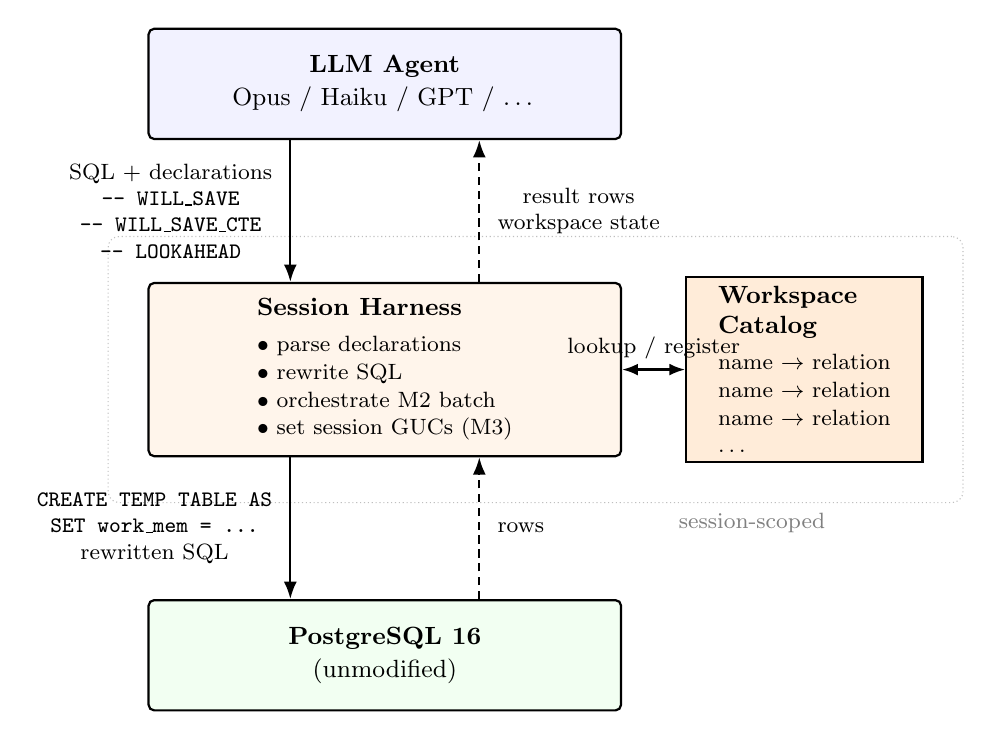
\begin{tikzpicture}[
    font=\small,
    node distance=10mm and 16mm,
    %% component styles
    agent/.style={
        draw, rounded corners=2pt, thick,
        minimum width=60mm, minimum height=14mm,
        align=center, fill=blue!5
    },
    harness/.style={
        draw, rounded corners=2pt, thick,
        minimum width=60mm, minimum height=22mm,
        align=left, fill=orange!8
    },
    catalog/.style={
        draw, thick,
        minimum width=30mm, minimum height=22mm,
        align=left, fill=orange!15
    },
    db/.style={
        draw, rounded corners=2pt, thick,
        minimum width=60mm, minimum height=14mm,
        align=center, fill=green!5
    },
    %% arrow styles
    flow/.style={-{Latex[length=2.2mm]}, thick},
    flowback/.style={-{Latex[length=2.2mm]}, thick, densely dashed},
    bidir/.style={{Latex[length=2mm]}-{Latex[length=2mm]}, thick},
    %% label styles
    lbl/.style={font=\footnotesize, align=center}
]

    %% --- nodes ------------------------------------------------
    \node[agent]   (agent)  {\textbf{LLM Agent} \\[1pt] \small Opus / Haiku / GPT / \ldots};

    \node[harness] (harness) [below=18mm of agent] {%
        \textbf{Session Harness}\\[2pt]
        \footnotesize $\bullet$ parse declarations\\[-1pt]
        \footnotesize $\bullet$ rewrite SQL\\[-1pt]
        \footnotesize $\bullet$ orchestrate M2 batch\\[-1pt]
        \footnotesize $\bullet$ set session GUCs (M3)
    };

    \node[catalog] (cat) [right=8mm of harness] {%
        \textbf{Workspace}\\
        \textbf{Catalog}\\[2pt]
        \footnotesize name $\to$ relation\\[-1pt]
        \footnotesize name $\to$ relation\\[-1pt]
        \footnotesize name $\to$ relation\\[-1pt]
        \footnotesize \ldots
    };

    \node[db] (db) [below=18mm of harness] {\textbf{PostgreSQL 16} \\[1pt] \small (unmodified)};

    %% --- arrows: Agent <-> Harness ----------------------------
    \draw[flow] ($(agent.south) + (-12mm,0)$) --
        node[lbl, left=1mm, pos=0.5] {
            SQL + declarations\\
            \ttfamily\footnotesize
            -- WILL\_SAVE\\
            \ttfamily\footnotesize
            -- WILL\_SAVE\_CTE\\
            \ttfamily\footnotesize
            -- LOOKAHEAD
        }
        ($(harness.north) + (-12mm,0)$);

    \draw[flowback] ($(harness.north) + (12mm,0)$) --
        node[lbl, right=1mm, pos=0.5] {
            result rows\\
            workspace state
        }
        ($(agent.south) + (12mm,0)$);

    %% --- arrows: Harness <-> Workspace Catalog ----------------
    \draw[bidir] (harness.east) -- node[lbl, above, pos=0.5] {lookup / register} (cat.west);

    %% --- arrows: Harness <-> PostgreSQL -----------------------
    \draw[flow] ($(harness.south) + (-12mm,0)$) --
        node[lbl, left=1mm, pos=0.5] {
            \ttfamily\footnotesize CREATE TEMP TABLE AS\\
            \ttfamily\footnotesize SET work\_mem = \ldots\\
            rewritten SQL
        }
        ($(db.north) + (-12mm,0)$);

    \draw[flowback] ($(db.north) + (12mm,0)$) --
        node[lbl, right=1mm, pos=0.5] {rows}
        ($(harness.south) + (12mm,0)$);

    %% --- session boundary (optional visual grouping) ----------
    \begin{pgfonlayer}{background}
        \node[draw=gray!50, densely dotted, rounded corners, inner sep=5mm,
              fit=(harness) (cat), label={[gray, font=\footnotesize]below right:{session-scoped}}] {};
    \end{pgfonlayer}

\end{tikzpicture}

\caption{Concord architecture. The agent emits SQL queries annotated with declarations (\texttt{WILL\_SAVE}, \texttt{WILL\_SAVE\_CTE}, \texttt{LOOKAHEAD}). The session harness parses declarations, registers materialized results in the workspace catalog, rewrites subsequent queries to reference them, and issues queries to an unmodified PostgreSQL~16. Dashed arrows denote data flow back to the agent.}
\label{fig:system}
\end{figure*}

The separation of concerns between harness and database is deliberate. Placing the protocol logic in a session-level harness, rather than in the database itself, keeps the database unmodified and keeps the protocol portable across database systems. The cost of this decision is that the harness cannot intervene in the query planner; the benefit is that the protocol can be deployed without extensions, planner patches, or binary modifications. All optimizations Concord performs are expressible as SQL-level rewrites, \texttt{CREATE TEMP TABLE} statements, and session-level GUC adjustments.

A \emph{session} is a bounded, ordered sequence of queries and declarations emitted by a single agent in service of a single analytical task. Sessions are the scope at which the workspace exists: when the session terminates, the workspace is dropped, and no state persists between sessions. This scoping is critical for the legality argument developed below---it bounds the surface over which the harness must reason about correctness.

\subsection{The Session Workspace}
\label{sec:protocol:workspace}

The workspace is a mutable set of named, materialized relations, each derived from a prefix of the session's query history. Formally, let a session $S$ be a sequence $S = \langle q_1, q_2, \ldots, q_n \rangle$ of queries, with declarations attached to individual queries. The workspace $W_i$ after query $q_i$ is a function
\[
W_i : \text{Name} \to \text{Relation}
\]
mapping declared names (e.g., \texttt{genre\_year\_ratings}) to stored relations (PostgreSQL temporary tables). The workspace evolves by two operations:

\begin{itemize}
\item \textbf{Register.} When query $q_i$ carries a \texttt{WILL\_SAVE} declaration with name $n$, the harness executes $q_i$ as \texttt{CREATE TEMP TABLE $n$ AS $q_i$} and registers $n \mapsto \text{relation}(n)$ in $W_i$.
\item \textbf{Resolve.} When query $q_j$ (for $j > i$) references $n$, the harness resolves the reference to the materialized relation.
\end{itemize}

Each materialized relation in the workspace is an immutable snapshot of the result at registration time. Concord does not maintain workspace entries under updates to the underlying tables; the assumption is that the underlying data is stable for the duration of an analytical session, which is consistent with the benchmark workloads we consider and with most practical agent-analytics scenarios. Relaxing this assumption is future work (Section~\ref{sec:discussion}).

\subsection{Declarations}
\label{sec:protocol:declarations}

Concord defines three declaration types. Each is expressed as a SQL comment prefixing the query it applies to, requiring no changes to PostgreSQL's parser or wire protocol.

\subsubsection{M1: Declared Materialization}
\label{sec:protocol:m1}

Two forms:

\begin{verbatim}
-- WILL_SAVE: <name> "<description>"
<query>
\end{verbatim}
declares that the result of \texttt{<query>} will be reused in subsequent queries of the session.

\begin{verbatim}
-- WILL_SAVE_CTE: <name> "<description>" cte=<cte_name>
WITH <cte_name> AS (<cte_body>)
<outer_query>
\end{verbatim}
declares that the body of the named CTE within a larger query is the reusable fragment, not the full query result. This form is important empirically: in our trace data, 10 of 15 M1-firing sessions used SAVE\_CTE, reflecting a common agent pattern of wrapping an expensive base in a CTE for immediate use and future reuse.

\paragraph{Legality condition.}
Given \texttt{WILL\_SAVE} on $q_i$, the harness is entitled to materialize $q_i$'s result as a physical temporary relation on first execution, without waiting for recurrence to justify the materialization cost. This is not safe under inferred intent: an observation-based system cannot know, at the first execution of $q_i$, whether $q_i$'s result will be reused or discarded, and the upfront materialization cost is unrecoverable if reuse does not materialize. Under declared intent, the agent takes responsibility for the declaration's accuracy.

\paragraph{What it enables.}
The immediate benefit is elimination of the double-execution cost incurred by post-hoc save: without a prior declaration, the agent must run $q_i$ to see its result, then issue a separate \texttt{workspace.save()} call that re-executes $q_i$ to materialize it. Pre-hoc \texttt{WILL\_SAVE} materializes during the first execution, saving one full execution of the base query. For the IMDB sessions in Section~\ref{sec:eval}, this corresponds to \TODO{X}s of redundant work per session.

\subsubsection{M2: Lookahead-Informed Multi-Query Optimization}
\label{sec:protocol:m2}

\begin{verbatim}
-- LOOKAHEAD: 3
-- q1: <query_1>
-- q2: <query_2>
-- q3: <query_3>
-- diff: q1 vs q2 WHERE year, q2 vs q3 GROUP BY
\end{verbatim}
The agent declares its next $k$ queries ($k = 2{-}5$ in our implementation) before issuing any of them, optionally identifying the differences between them via a \texttt{diff} clause.

\paragraph{Legality condition.}
Given a \texttt{LOOKAHEAD} declaration of queries $q_{i+1}, \ldots, q_{i+k}$, the harness is entitled to: (i) identify common subexpressions across the declared window; (ii) construct a shared physical plan that materializes these subexpressions once, with physical properties (sort order, partial aggregates, covering columns) synthesized from the union of access patterns across the declared queries; and (iii) execute the shared plan once, satisfying each declared query from the shared result. Under inferred intent, steps (i)--(iii) are unsafe at the moment $q_{i+1}$ arrives, because the database does not know that $q_{i+2}, \ldots$ will be issued at all.

\paragraph{What it enables.}
Three classes of optimization become legal:

\begin{itemize}
\item \emph{Shared scan.} If $q_{i+1}, \ldots, q_{i+k}$ share a common table scan with overlapping filters, the harness executes the scan once and feeds results to each query's downstream operations. This subsumes M1 as a special case (where the shared subexpression is the entire base query) and extends it to cases where the agent has not explicitly declared a save but has declared a lookahead.
\item \emph{Physical-property synthesis.} If all declared queries group by the same key, the shared materialization can be sorted on that key, enabling merge-based aggregations downstream. If all declared queries compute the same aggregate function over overlapping groups, a partial-aggregate materialization is legal.
\item \emph{Covering column selection.} The shared materialization includes only the columns that appear in the union of projection, filter, and grouping clauses across declared queries, reducing I/O relative to a naive full-row materialization.
\end{itemize}

The \texttt{diff} clause, when present, identifies exactly which predicates or grouping dimensions vary across lookahead queries, allowing the harness to precompute the shared portion and parameterize only the variant portion.

\subsubsection{M3: Reuse-Aware Physical Tuning}
\label{sec:protocol:m3}

M3 is not a distinct declaration in the sense of M1 and M2; it is a set of harness behaviors activated by the declarations of M1 and M2. Specifically, given the declared workspace contents (via M1) and declared access patterns (via M2), the harness sets session-level GUCs---\texttt{work\_mem}, \texttt{enable\_parallel\_append}, \texttt{jit\_above\_cost}---to values appropriate for the declared workload characteristics, and optionally clusters or sorts materialized temporary relations to match declared access patterns. The legality argument for M3 is subsumed by those of M1 and M2: it is what the harness does with the declarations it has already received.

\paragraph{What it enables.}
For the full-scan analytical workloads that dominate agent sessions, the primary wins are: (i) sizing \texttt{work\_mem} to fit the declared temp-table's hash aggregation, avoiding spill; (ii) enabling parallelism on temp-table scans; and (iii) sorting the temp table on the dominant declared group-by key, converting hash aggregations to merge aggregations. Conventional indexing is \emph{not} part of M3; our measurements in Section~\ref{sec:eval} show that indexes on temporary workspace relations do not help and sometimes hurt this workload.

\subsection{Cost Model: Lookahead Is Never Worse}
\label{sec:protocol:costmodel}

We sketch a cost-model result establishing that under faithful declarations, lookahead-informed execution is never worse than ad-hoc per-query execution. The full formal development is deferred to an extended version; the sketch below names the assumptions and the result.

\paragraph{Setup.}
Let $C(q)$ denote the execution cost of query $q$ under PostgreSQL's cost model, executed in isolation. Let $C_{\text{shared}}(q_{i+1}, \ldots, q_{i+k})$ denote the cost of executing a shared-plan materialization of the $k$ declared queries followed by the per-query residual computations over the shared result. Let $\tilde{C}(q)$ denote the cost of query $q$ executed against the shared materialization (typically $\tilde{C}(q) \ll C(q)$ because the expensive join-and-filter base is already materialized).

\paragraph{Assumptions.}
\textbf{(A1)} The agent's lookahead declaration is faithful: declared queries $q_{i+1}, \ldots, q_{i+k}$ are exactly the queries the agent will subsequently issue, in the declared order.
\textbf{(A2)} The harness's common-subexpression identification is correct: the shared subexpression identified across the window is a subexpression of each declared query.
\textbf{(A3)} PostgreSQL's cost model is monotone: executing a query against a materialized subexpression costs no more than executing it from scratch.

\paragraph{Claim (informal).}
Under (A1)--(A3), for any lookahead window $\langle q_{i+1}, \ldots, q_{i+k}\rangle$,
\[
C_{\text{shared}}(q_{i+1}, \ldots, q_{i+k}) \;\leq\; \sum_{j=1}^{k} C(q_{i+j}).
\]

\paragraph{Proof sketch.}
The shared plan computes the common subexpression once (cost $C_{\text{common}}$) and then each residual (cost $\tilde{C}(q_{i+j})$ for $j = 1, \ldots, k$). The per-query baseline pays $C(q_{i+j})$ for each query, which, under (A2)--(A3), satisfies $C(q_{i+j}) \geq C_{\text{common, j}} + \tilde{C}(q_{i+j})$ where $C_{\text{common, j}}$ is the cost of computing the common subexpression within query $q_{i+j}$. Summing over $j$ and noting that the shared plan computes $C_{\text{common}}$ once rather than $k$ times yields the inequality.
\qed

\paragraph{What this result does and does not establish.}
It establishes that faithful lookahead declarations cannot \emph{worsen} session cost relative to per-query execution, modulo the correctness of the harness's subexpression identification. It does \emph{not} establish a lower bound on the speedup, which depends on the weight of the shared subexpression relative to the residuals---an empirical question addressed in Section~\ref{sec:eval}. It also does not address unfaithful declarations: if the agent declares $q_{i+2}$ but never issues it, the shared materialization's cost is wasted on the unused residual. Empirically (Section~\ref{sec:eval}), we find that agents achieve \mTwoPrecision precision on declared queries, so the unfaithful-declaration regime is rare; we discuss adversarial cases in Section~\ref{sec:discussion}.

\section{Implementation}
\label{sec:impl}

\TODO{Draft after pre-hoc save and M2 build are complete. Outline:}

\subsection{Session Harness Architecture}
\TODO{harness as a Python process; SQL pre-processor; workspace catalog in PL/pgSQL; interaction flow diagram if helpful}

\subsection{Declaration Parsing}
\TODO{comment-based parsing, grammar, handling of malformed declarations}

\subsection{Pre-Hoc Save Implementation}
\TODO{WILL\_SAVE rewrite to CREATE TEMP TABLE AS; WILL\_SAVE\_CTE via sqlglot CTE extraction; handling of nested CTEs}

\subsection{Lookahead Execution Engine}
\TODO{common-subexpression identification algorithm; physical-property synthesis heuristics; plan construction}

\subsection{Physical Tuning Controller}
\TODO{GUC adaptation logic; clustering decisions; partial-aggregate synthesis}

\subsection{Extension-Free PostgreSQL Integration}
\TODO{why no extensions needed; what we gave up by staying at the SQL layer; what this buys us in portability}

\section{Evaluation}
\label{sec:eval}

\TODO{Draft after all experiments run. Outline below reflects the locked study structure.}

\subsection{Experimental Setup}
\TODO{hardware, PG16 config, agent models, temperatures, query caps, benchmark datasets (IMDB/JOB and curated InsightBench subset)}

\subsection{E1: End-to-End Headline on InsightBench}
\TODO{Primary headline result. Protocol vs.\ Baseline A across \placeholder{} curated tasks. Table of per-task session time and quality-rubric agreement.}

\subsection{E2: End-to-End Mechanism Study on IMDB}
\TODO{Per-scenario session time breakdown across 20 reps. Table below is the structure; numbers update when pre-hoc and M2 land.}

%% Placeholder table showing the result structure; numbers from current post-hoc M1 data
\begin{table}[h]
\centering
\small
\caption{IMDB session-time breakdown, M1 post-hoc implementation (20 reps across 10 scenarios). \TODO{Replace with pre-hoc + M2 + M3 numbers when measured.}}
\label{tab:e2-imdb}
\begin{tabular}{lrrrr}
\toprule
Scenario & With M1 (s) & Baseline (s) & Savings (s) & Speedup \\
\midrule
1.\ Genre Evolution & 29.8 & 51.1 & 21.3 & 1.72$\times$ \\
2.\ Director Career & 393.5 & 496.8 & 103.3 & 1.26$\times$ \\
3.\ Company Genre & 34.3 & 43.2 & 8.9 & 1.26$\times$ \\
4.\ Cast Size & 100.7 & 117.0 & 16.4 & 1.16$\times$ \\
5.\ Co-Production & 36.9 & 51.1 & 14.2 & 1.38$\times$ \\
6.\ Franchise & 10.9 & 15.5 & 4.5 & 1.41$\times$ \\
7.\ Writer-Director & 18.7 & 24.7 & 6.0 & 1.32$\times$ \\
8.\ Actor Archetypes & 198.9 & 319.4 & 120.5 & 1.61$\times$ \\
9.\ Spillover & 235.1 & 256.0 & 20.9 & 1.09$\times$ \\
10.\ Budget & 16.6 & 23.4 & 6.8 & 1.41$\times$ \\
\midrule
\textbf{TOTAL} & \textbf{1075.3} & \textbf{1398.1} & \textbf{322.7} & \textbf{\imdbSpeedupPostHoc} \\
\bottomrule
\end{tabular}
\end{table}

\subsection{E3: Per-Mechanism Ablation}
\TODO{M1-only / M1+M2 / M1+M2+M3 / full protocol on IMDB. Bar chart or stacked bar.}

\subsection{E4: Agent Adoption and Declaration Faithfulness}
\TODO{Voluntary adoption rates, SAVE\_CTE distribution, M2 precision; documented failure mode ``iteration on base''}

Observed across the 20-rep IMDB suite under M1 post-hoc:
\begin{itemize}
\item M1 adoption: \adoptionRate voluntary save rate (15/20 reps).
\item SAVE\_CTE dominance: \saveCteRate of reps use SAVE\_CTE specifically.
\item M2 declaration rate: \mTwoDeclRate (9/20 reps).
\item M2 precision: \mTwoPrecision of declared variants actually issued.
\item Task completion: \taskCompletionIMDB.
\end{itemize}

\subsection{E5: Intra- vs.\ Inter-Query Reuse}
\TODO{Single-ref vs.\ multi-ref CTE subset. Measures Concord's contribution beyond PG16's built-in multi-ref CTE materialization.}

Current post-hoc numbers:
\begin{itemize}
\item Single-reference reuse subset (44 queries): \imdbSingleRefSpeedup speedup. PG16 would inline the CTE; Concord's materialization is where the win comes from.
\item Multi-reference subset (25 queries): \imdbMultiRefSpeedup speedup. PG16 already materializes; Concord's delta is smaller (but still positive, reflecting physical-property benefits from M3).
\end{itemize}

\subsection{E6: Sensitivity}
\TODO{Lookahead depth $k \in \{1,2,3,5\}$; agent capability axis (Opus / Haiku / mid-tier); data scale (IMDB 10\% / 100\%).}

\subsection{Quality Evaluation}
\TODO{Pre-registered rubric, blinded human grading of paired outputs, LLM-judge cross-validation, symmetric reporting (agreement / protocol-wins / baseline-wins rates).}

\section{Discussion}
\label{sec:discussion}

\TODO{Draft last. Candidate threads:}

\subsection{Failure Modes}
\TODO{iteration-on-base pattern (documented in IMDB); adversarial / unfaithful declarations; workloads without reuse structure}

\subsection{Generalization Beyond PostgreSQL}
\TODO{The protocol is SQL-level. What would it take to port to DuckDB, Snowflake, BigQuery? What breaks?}

\subsection{Transparent Query Rewriting (Future Work)}
\TODO{The M3-as-originally-scoped ``transparent rewriting'' idea --- detecting reuse opportunities the agent did not declare and rewriting queries behind the agent's back --- is deferred as future work. Briefly motivate why the current paper stops at declared intent.}

\subsection{Data Staleness and Long Sessions}
\TODO{workspace assumes stable underlying data; sessions that span updates need invalidation; briefly discuss what that would look like}

\subsection{Protocol in a World of Stronger Agents}
\TODO{as agents become better SQL writers, does the protocol become less valuable or more? Argument: more, because better agents declare more faithfully.}

\section{Conclusion}
\label{sec:conclusion}

\TODO{Draft last. One-paragraph recap of thesis, mechanisms, headline results. One-paragraph forward-looking statement about agent-cooperative databases as a design space.}


\bibliographystyle{ACM-Reference-Format}
\bibliography{bib/refs}

\end{document}
